%%===========================================================%%
%%                                                           %%
%%                        CORRECTIONS                        %%
%%                                                           %%
%%===========================================================%%


\chapter{Corrections}\label{chap:corrections}

\section{Method of corrections application}\label{sec:correctionProcedure}
\begin{equation}
  \frac{d\sigma}{dq} = \frac{1}{\Delta q} \times \frac{1}{\varepsilon} \times \frac{N^{\mathit{w}}-N^{\mathit{w}}_\textrm{bkgd}}{\mathit{L}_{\textrm{int}}^{\textrm{eff}}}
\end{equation}

%remembed about accounting for RP trigger eff!!!
\begin{equation}\label{eq:effectiveLumi}
	\mathit{L}_{\textrm{int}}^{\textrm{eff}} = \sum\limits_{\textrm{run}}\mathit{L}_{\textrm{int}}^{\textrm{run}} \times \epsilon_{\textrm{veto}}(L^{\textrm{run}})
\end{equation}
% \left(\epsilon_{\textrm{veto}}^{\textrm{online}} \oplus \epsilon_{\textrm{veto}}^{\textrm{offline}}(L_{\textrm{run}}) \right)

\begin{equation}
	\varepsilon = \epsilon_{\textrm{\tiny ET/IT}} \times \epsilon_{\textrm{vrtx}}(q) \times \epsilon_{\ref{enum:CutZVx}} \times \epsilon_{\ref{enum:CutDeltaZVx}} \times \epsilon_{\ref{enum:CutMissingPt}} \times \epsilon_{\textrm{\tiny PID}}(q)
\end{equation}

\begin{equation}
	N^{\mathit{w}} = \sum\limits_{\textrm{event}}\mathit{w}_{\textrm{event}}
\end{equation}



\begin{equation}
	\mathit{w} = \left[\prod\limits_{\textrm{sign}} \epsilon_{\textrm{\tiny TOF}}(\textrm{sign}, \textrm{PID}, p_{T},z_{vx},\eta)  \times \prod\limits_{\textrm{sign}} \epsilon_{\textrm{\tiny TPC}}(\textrm{sign}, \textrm{PID}, p_{T},z_{vx},\eta) \times \prod\limits_{\textrm{side}}\epsilon_{\textrm{\tiny RP}}^{\textrm{side}}(p_{x},p_{y}) \right]^{-1},
\end{equation}
\[\textrm{sign}\in\{+,-\},~~\textrm{side}\in\{E,W\}\]
% ()




\section{Acceptances and efficiencies}

In this section we present calculation of all efficiencies except TPC track reconstruction and TOF hit reconstruction and matching efficiency, which were discussed and presented in Ref.~\cite{supplementaryNote}.

\subsection{Trigger efficiency}\label{sec:triggerEff}
\subsubsection{Online veto (BBC-small and ZDC veto)}\label{sec:onlineVetoEff}

Vetoeing signal in BBC-small and ZDC detectors on both sides of STAR was implemented in the logic of RP\_CPT2 trigger. Common correction of the online and offline vetoes which is used in the correction procedure explained in Sec.~\ref{sec:correctionProcedure} is presented in. Sec.~\ref{sec:onlineAndOfflineVetoEff}. However, to help quantifiy effect of just the online vetoes in BBC-small and ZDCs we show the Fig.~\ref{fig:onlineVetoEff} with the efficiency of the joint BBC-small and ZDC veto as a function of the instantaneous luminosity calculated from the zero-bias data. Details of the way the efficiency was calculated as well as description of the data in the Figure is the same as explained in Sec.~\ref{sec:onlineAndOfflineVetoEff}.
%---------------------------
\begin{figure}[ht!]
\centering%
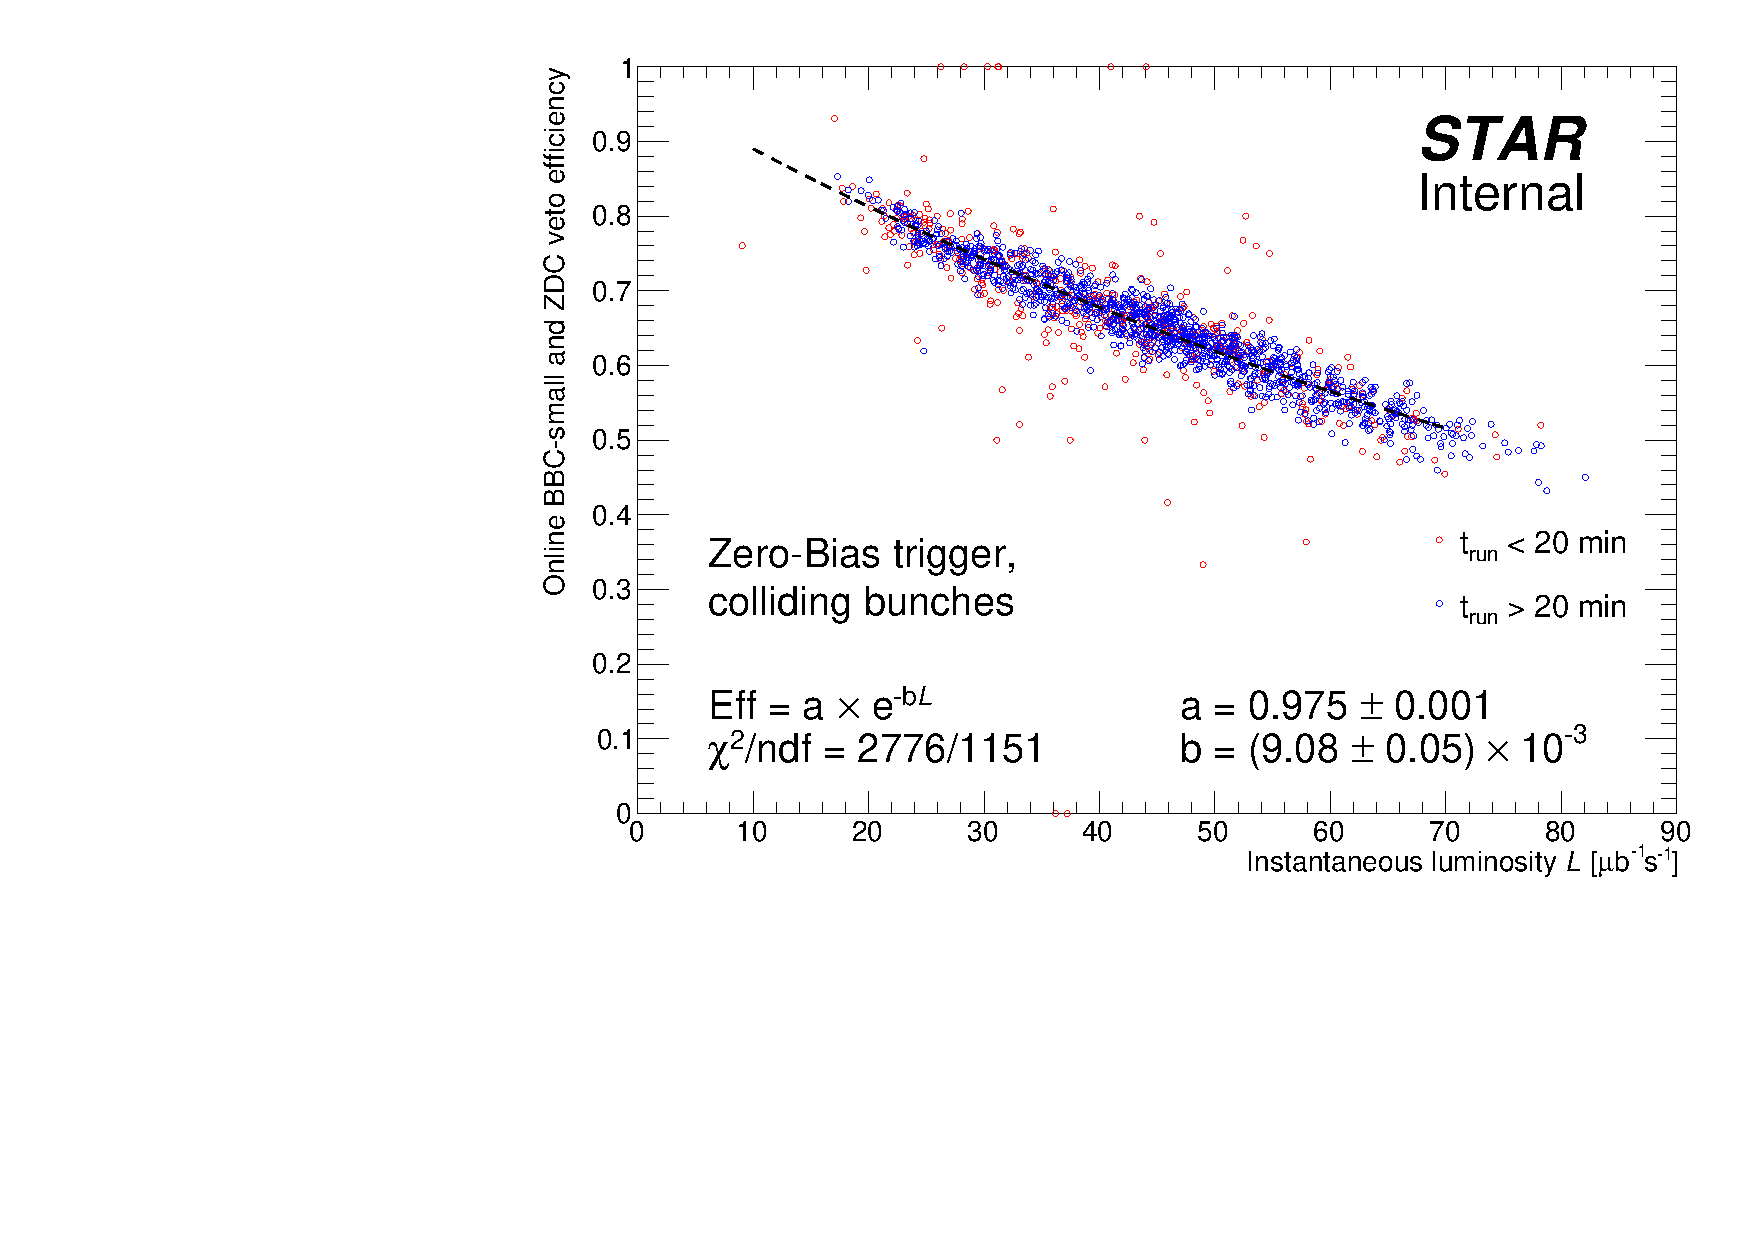
\includegraphics[width=0.65\linewidth,page=1]{graphics/corrections/OnlineVetoEffVsInstLumi_graph.pdf}%
\caption{Overall efficiency of the online BBC-small and ZDC veto as a function of instantaneous luminosity.}\label{fig:onlineVetoEff}%
\end{figure}
%---------------------------

\subsubsection{RP triggering efficiency}\label{sec:rpTrigEff}

Based on preliminary studies preformed during data taking using fast offline data (MuDst) we concluded that the RP triggering efficiency is very close to 100~\% and eventual correction (which is going to be evaluated) is much smaller than overall systematic uncertainty. For the time being we assume that
\begin{equation}
\mbox{\LARGE$\varepsilon$}\left(\TRE\land\TRW\right) =  \mbox{\LARGE$\varepsilon$}\left(\TRW\right) \times \mbox{\LARGE$\varepsilon$}\left(\TRE\right) = 1.
\end{equation}


% Wydajnosc samego trygerowania
% \begin{equation}
% \mbox{\LARGE$\varepsilon$}\left(\TRE\land\TRW\right) = \mbox{\LARGE$\varepsilon$}\left(\TRE\right) \times \mbox{\LARGE$\varepsilon$}\left(\TRW\right),
% \end{equation}
% \begin{equation}
% \mbox{\LARGE$\varepsilon$}\left(\TRE\right) = \mbox{\LARGE$\varepsilon$}\left(\TRE_{1}\vee\TRE_{2}\right),~~~~\mbox{\LARGE$\varepsilon$}\left(\TRW\right) = \mbox{\LARGE$\varepsilon$}\left(\TRW_{1}\vee\TRW_{2}\right),
% \end{equation}
% dobrze bedzie policzyc już z danych, najlepiej elastycznych (ale można też z CD) patrzac jak czesto stacje z dobrymi sladami maja sygnal trygerowy.
% 
% \begin{equation}\begin{split}
% \mbox{\LARGE$\varepsilon$}\left(\TRW\right) = \mbox{\LARGE$\varepsilon$}\left(\TRW\left|\RPE\&\RPW\&~!\TRNE\&~!\TRNW\right.\right) = \mbox{\LARGE$\varepsilon$}\left(\TRW_{1}\vee\TRW_{2}\left|\RPE\&\RPW\&~!\TRNE\&~!\TRNW\right.\right)=\\
% =\mbox{\LARGE$\varepsilon$}\left(\TRW_{1}\left|\RPE\&\RPW\&~!\TRNE\&~!\TRNW\right.\right)+\mbox{\LARGE$\varepsilon$}\left(\TRW_{2}\left|\RPE\&\RPW\&~!\TRNE\&~!\TRNW\right.\right)+\\-\mbox{\LARGE$\varepsilon$}\left(\TRW_{1}\land\TRW_{2}\left|\RPE\&\RPW\&~!\TRNE\&~!\TRNW\right.\right)~~~~~\text{(analogicznie po stronie EAST)}
% \end{split}\end{equation}


\subsubsection{Up and Down RP combination veto (due to dead material)}\label{sec:rpDeadMat}

Probability that secondaries induced by proton with successfully reconstructed and selected RP track generate a trigger signal in the other RP branch on the same side was calculated using the embedded MC (see Sec.~6.3 in Ref.~\cite{supplementaryNote} for details of RP simulation in Geant4). Forward protons from CEP process provided by GenEx~\cite{GenEx} were simultaneously generated from the interaction point spatially distributed the same as in the data. MC samples for all runs with RP\_CPT2 triggers were produced to account for non-constant positions of the RP detectors throughout the run 15. Number of simulated events for each run was proportional to number of RP\_CPT2 triggers in given run. The angular divergence of the beams was also simulated.

The discussed probability, $\mathcal{P}_{\text{DM~veto}}^{\text{side}}$, was calculated as a probability that a MC-trigger signal is present in the branch on given side other than east and west branches where primary forward protons are expected from their initial momenta, under condition that these east and west branches detect a MC-trigger signal and there is no veto due to simultaneous ET\&IT trigger bits in the overlayed data (no pile-up veto). By MC-trigger we understand the trigger signal reconstructed solely from the simulated data (not from the data embedded into).

Technically the $\mathcal{P}_{\text{DM~veto}}^{\text{side}}$ was obtained in the following procedure:
\begin{enumerate}
  \item No simultaneous ET\&IT trigger bits were allowed in the data of an event that simulated signal was embedded into.
	\item It was verified if there are MC-trigger signals in east and west branches that the primary forward protons were expected to reach based on their $p_{y}$ ($p_{y}>0$ - branch UP, $p_{y}<0$ - branch DOWN). These events formed $set~A$.
	\item Events with the MC-trigger signal in RP branch other than the branch with MC-trigger signal expected from proton $p_{y}$ on given side formed $set~B$.
	\item The probability was determined by the ratio of histograms from $set~B$ and $set~A$:
	\begin{equation}\label{eq:rpDeadMatProb}
	\begin{split}
 \mathcal{P}_{\text{DM~veto}}^{\text{side}}(p_{x}, p_{y}, z_{\text{vtx}}) = \mbox{\LARGE$\varepsilon$}^{\text{side}}\left(\Vdm\left|!\Vpu\land\TRE\land\TRW\right.\right) = ~~~~~~~~~~~~~~~~~~~~~~~~~~~~~~~~~~~~~~\\~~~~~~~~~~~~~~~~~~~~~~~~~~~~~~~ =%
 \frac{(p_{x}, p_{y}, z_{\text{vtx}})~\text{histogram for protons from}~set~B}{(p_{x}, p_{y}, z_{\text{vtx}})~\text{histogram for protons from}~set~A}
 \end{split}
  \end{equation}
	
\end{enumerate}

It should be noted that the momentum components $(p_{x}, p_{y})$ were taken from the proton with accounted effect of the beam divergence (after the original initial momentum smearing). Sample probability of a dead-material-induced veto is shown in Fig.~\ref{fig:sampleRpDeadMatVeto}, with all the remaining results contained in Appendix~\ref{appendix:rpEff}.

The efficiency of the discussed veto which is finally used to correct the data is opposite of the veto probability, namely
\begin{equation}
 \mbox{\LARGE$\epsilon$}_{\text{DM~veto}}^{\text{side}} = 1 - \mathcal{P}_{\text{DM~veto}}^{\text{side}}.
\end{equation}


%---------------------------
\begin{figure}[ht!]
\centering%
\parbox{0.4725\textwidth}{%
  \centering%
  \includegraphics[width=\linewidth,page=3]{graphics/corrections/mcDeadMatProbPxPy.pdf}\label{fig:sampleDeadMatVetoProb}
}%
\quad%
\parbox{0.4725\textwidth}{%
    \caption[Sample probability of ET\&IT trigger veto due to forward proton interaction with dead material.]{Sample probability of ET\&IT trigger veto due to forward proton interaction with dead material. Results were obtained from forward proton MC simulation embedded into zero-bias data.}\label{fig:sampleRpDeadMatVeto}%
}
\end{figure}
%---------------------------





\subsection{Selection efficiency}\label{sec:cutsEff}
\subsubsection{TPC \texorpdfstring{$z$}{z}-vertex cut~(\ref{enum:CutZVx})}

Removing from analysis specific range of $z$-positions of primary vertices effectively reduces accepted luminosity with respect to that delivered by the collider. This loss of luminosity has to be accounted when calculating the cross sections, which is the goal of presented analysis. Assuming that the distribution of $z_{\text{vtx}}$ of all primary interactions that take place when east and west beams overlap follows a normal distribution ($\mathcal{N}$), then the formula describing efficiency of the cut~\ref{enum:CutZVx} has the following form:
\begin{equation}\label{eq:zVtxCutEff}
 \mbox{\LARGE$\epsilon$}_{z_{\text{vtx}}} = \int\limits_{z_{\text{vtx}}^{\text{min}}}^{z_{\text{vtx}}^{\text{max}}} \mathcal{N}(z_{\text{vtx}}; \mu, \sigma)~\text{d}z_{\text{vtx}} = \frac{1}{2}\left[ \text{Erf}\left(\frac{z_{\text{vtx}}^{\text{max}} - \mu}{\sqrt{2}\sigma}\right) - \text{Erf}\left(\frac{z_{\text{vtx}}^{\text{min}} - \mu}{\sqrt{2}\sigma}\right) \right],
\end{equation}
where $z_{\text{vtx}}^{\text{min}}$ and $z_{\text{vtx}}^{\text{max}}$ are respectively minimum and maximum value of the longitudinal position of the vertex accepted in analysis (in our case these are -80~cm and 80~cm), and parameters $\mu$ and $\sigma$ are respectively the mean and standard deviation of the normal distribution:
\[\mu = \langle z_{\text{vtx}}\rangle,~~~~~~~~~~~~~~~\sigma = \sigma(z_{\text{vtx}}).\]

Real parameters of $z_{\text{vtx}}$ distribution were studied separately for every single fill of the collider. It is motivated by the fact that each fill of the machine is nearly independent from the previous thus the shape and position of $z_{\text{vtx}}$ may vary on fill by fill basis. We neglect possible changes within the fill (e.g. widening of the distribution due to intrabeam scattering etc.) arguing that this effect if expected to be smaller than the systematic uncertainties related to determination of position and width of $z_{\text{vtx}}$ distribution.

For every fill of RHIC the distribution of $z_{\text{vtx}}$ of single TOF vertices was prepared, as shown in Fig.~\ref{fig:sampleZVtxHist}. This distribution was fitted with the Gaussian function in a range $z_{\text{vtx}}\in[-120~\text{cm}, 120~\text{cm}]$. The output parameters of all fits were plotted as a function of the fill number, as shown in Fig.~\ref{fig:zVxMeanAndSigmaVsFillNumber}. The efficiency used in the correction procedure was calculated independetly for each fill using presented values of $\langle z_{\text{vtx}}\rangle$ and $\sigma(z_{\text{vtx}})$. Typical numerical value of this efficiency equals $\sim88\%$.

%---------------------------
\begin{figure}[ht!]% 
\centering%
\begin{minipage}{.4725\textwidth}%
  \centering%
  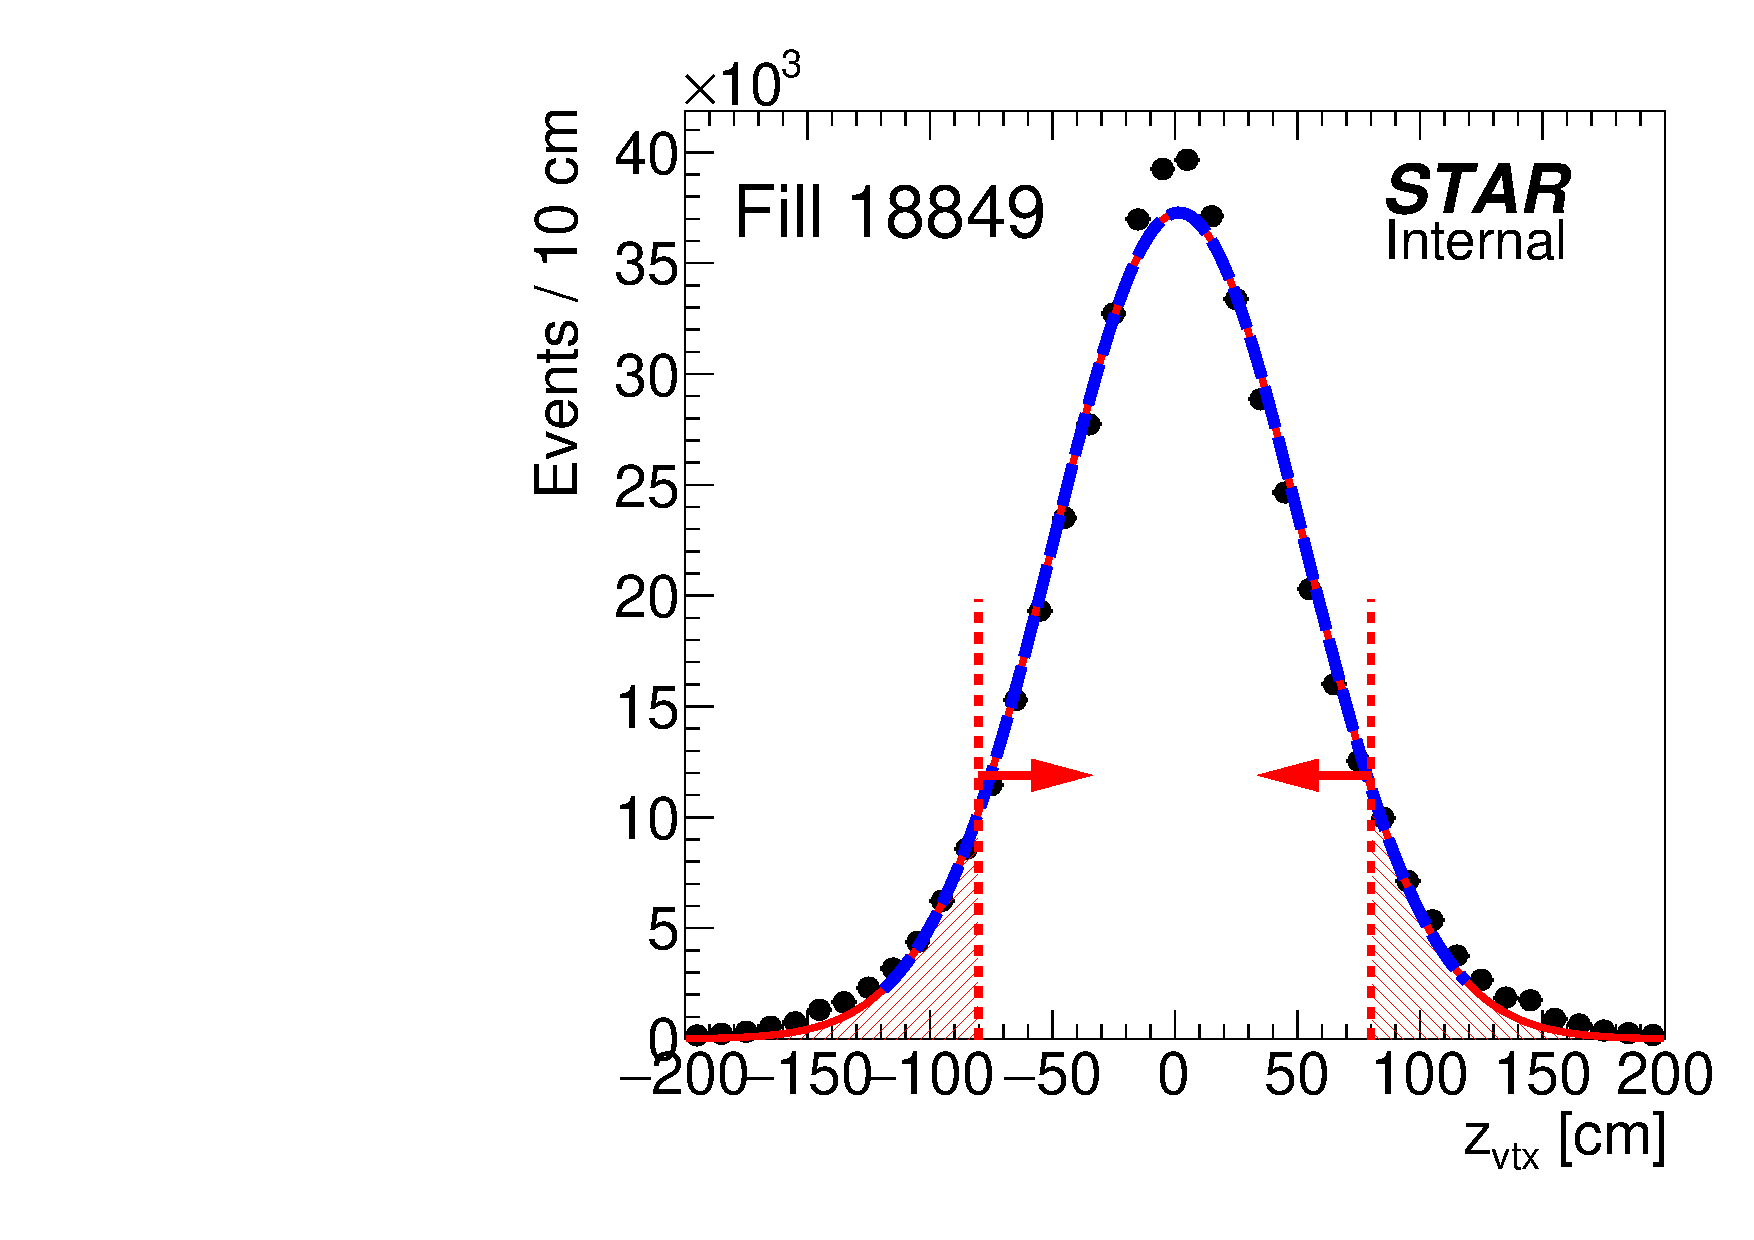
\includegraphics[width=\linewidth]{graphics/corrections/sampleZVtxHist.pdf}%
  \caption[Sample distribution of $z_{\text{vtx}}$ with fitted normal distribution.]{Sample distribution of $z_{\text{vtx}}$ of single TOF vertices together with the fit of normal distribution (dashed blue) extended outside the range of the fit (solid red). Hashed red area represents part of the distribution rejected by cut~\ref{enum:CutZVx} with the cut value marked with dashed red vertical lines and arrows.}\label{fig:sampleZVtxHist}
\end{minipage}% 
\quad\quad%
\begin{minipage}{.4725\textwidth}%
  \centering
  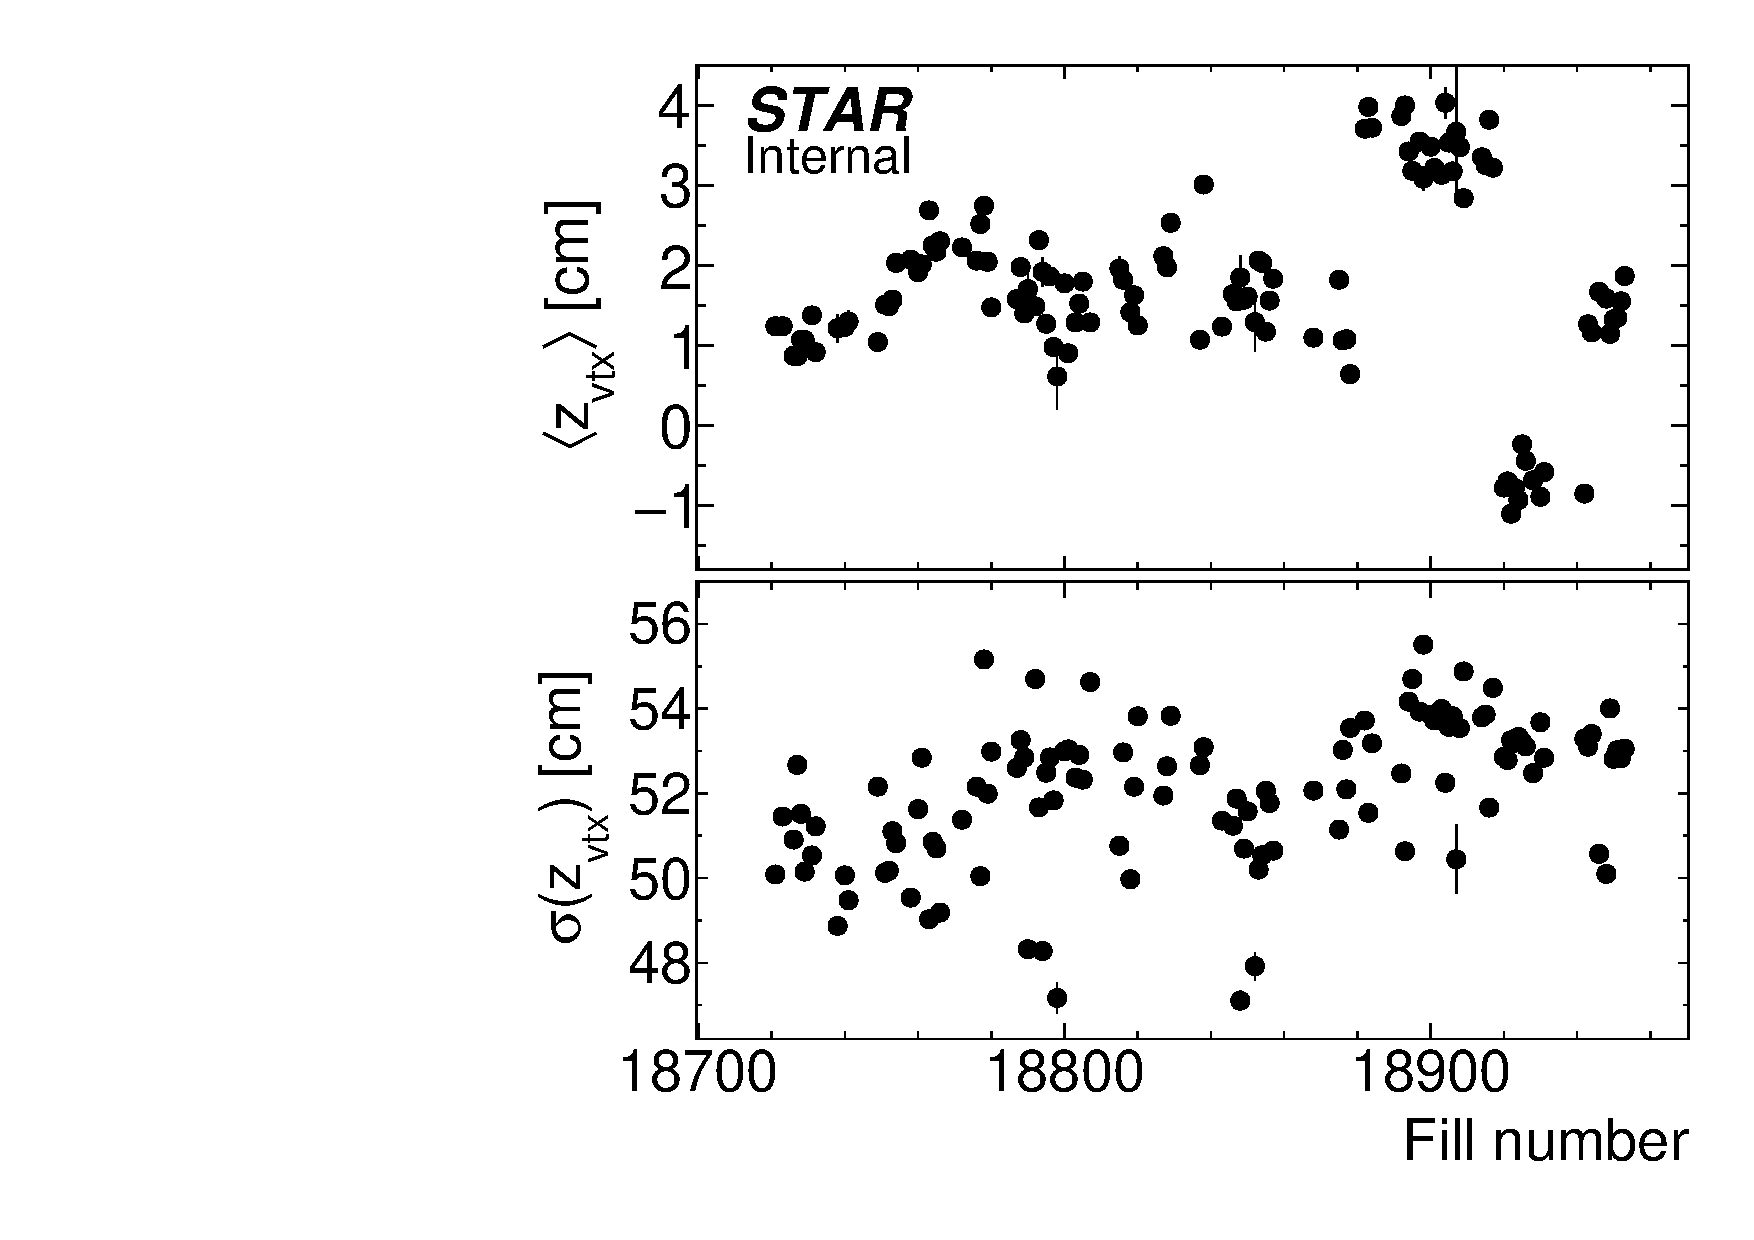
\includegraphics[width=\linewidth]{graphics/corrections/zVxMeanAndSigmaVsFillNumber.pdf}%
  \caption[Mean and width of the $z_{\text{vtx}}$ distribution as a function of the RHIC fill number.]{Mean (top panel) and width (bottom panel) parameters of the normal distribution obtained from a fit of normal distribution to $z_{\text{vtx}}$ distribution in a range $[-120~\text{cm}, 120~\text{cm}]$ for each RHIC fill as a function of the fill number.\newline}\label{fig:zVxMeanAndSigmaVsFillNumber}
\end{minipage}%
\end{figure}%
%---------------------------


\subsubsection{TPC-RP \texorpdfstring{$z$}{z}-vertex matching~(\ref{enum:CutDeltaZVx})}
\subsubsection{Primary vertices limit~(\ref{enum:CutPrimVx}), BBC-large veto~(\ref{enum:CutBbcLarge}), TOF clusters limit~(\ref{enum:CutTofClusters}) and Up and Down RP combination veto (due to pile-up)}\label{sec:onlineAndOfflineVetoEff}

Combined efficiency of the online veto in BBC-small and ZDC (Sec.~\ref{sec:onlineVetoEff}) and offline cuts (vetoes) on extra TPC-TOF vertices, extra TOF clusters, signal in BBC-large and simultaneous signal in Up and Down RPs, was calculated using the zero-bias data. For each run a fraction of events (for colliding bunches) was calculated in which all mentioned cuts would be satisfied in case of the CEP $\pi^{+}\pi^{-}$/$K^{+}K^{-}$/$p\bar{p}$ event (event would not be vetoed). One can tranform this prescription to simple formula below:

\begin{equation}
 \mbox{\LARGE$\epsilon$}^{\text{veto}}_{b_{E}b_{W}}=\dfrac{\splitdfrac{~~~~~\text{\#events in the run without TOF vertices, without signal in BBC-S, BBC-L, ZDC,}}{\text{RP branches other than} ~b_{E},~b_{W},~\text{and with no more than 1 reconstructed TOF cluster}}}{\text{\#events in the run}}
\end{equation}

In Fig.~\ref{fig:onlineAndOfflineVetoEff} this efficiency is presented as a function instantaneous luminosity delivered by the machine, for each combination of east and west RP branches. Result for each combination is nearly identical as the effect of ET\&IT trigger veto in RPs is not dominant, as well as trigger in all branches had similar acceptance. The data points were fitted with the exponential function (of the form containted in the figure) which reflects the fact that this efficiency should behave similar to the probability of lack of any interaction in the bunch crossing given by the Poisson distribution:
\begin{equation}\label{eq:poisson}
 \text{Pois}(0;\mu) = \frac{\mu^{0}}{0!} \times e^{-\mu} = e^{-\mu}.
\end{equation}
Comparison of the $\mu$ in Eq.~\eqref{eq:poisson} with the fit parameters in Fig.~\ref{fig:onlineAndOfflineVetoEff} leads to approximate determination of the average interaction probability per bunch crossing equal $0.2-0.9$. The result of the fit, $ \mbox{\LARGE$\epsilon$}^{\text{veto}}_{b_{E}b_{W}}(\mathcal{L})$, is finally used to correct measured data as described in Sec.~\ref{sec:correctionProcedure}. 

Comparison of efficiencies in Fig.~\ref{fig:onlineAndOfflineVetoEff} with similar efficiency in Fig.~\ref{fig:onlineVetoEff} demonstrates that offline selection has much smaller impact on the loss of signal events than online selection. It has to be underlined that online vetoes were necessary to set trigger purity to satisfactory level, as well as reduce prescale of the trigger.
%---------------------------
\begin{figure}[h]
\centering
\parbox{0.4725\textwidth}{
  \centering
  \begin{subfigure}[b]{\linewidth}
                \subcaptionbox{\label{fig:sampleBbcSmallAdcVsTac}}{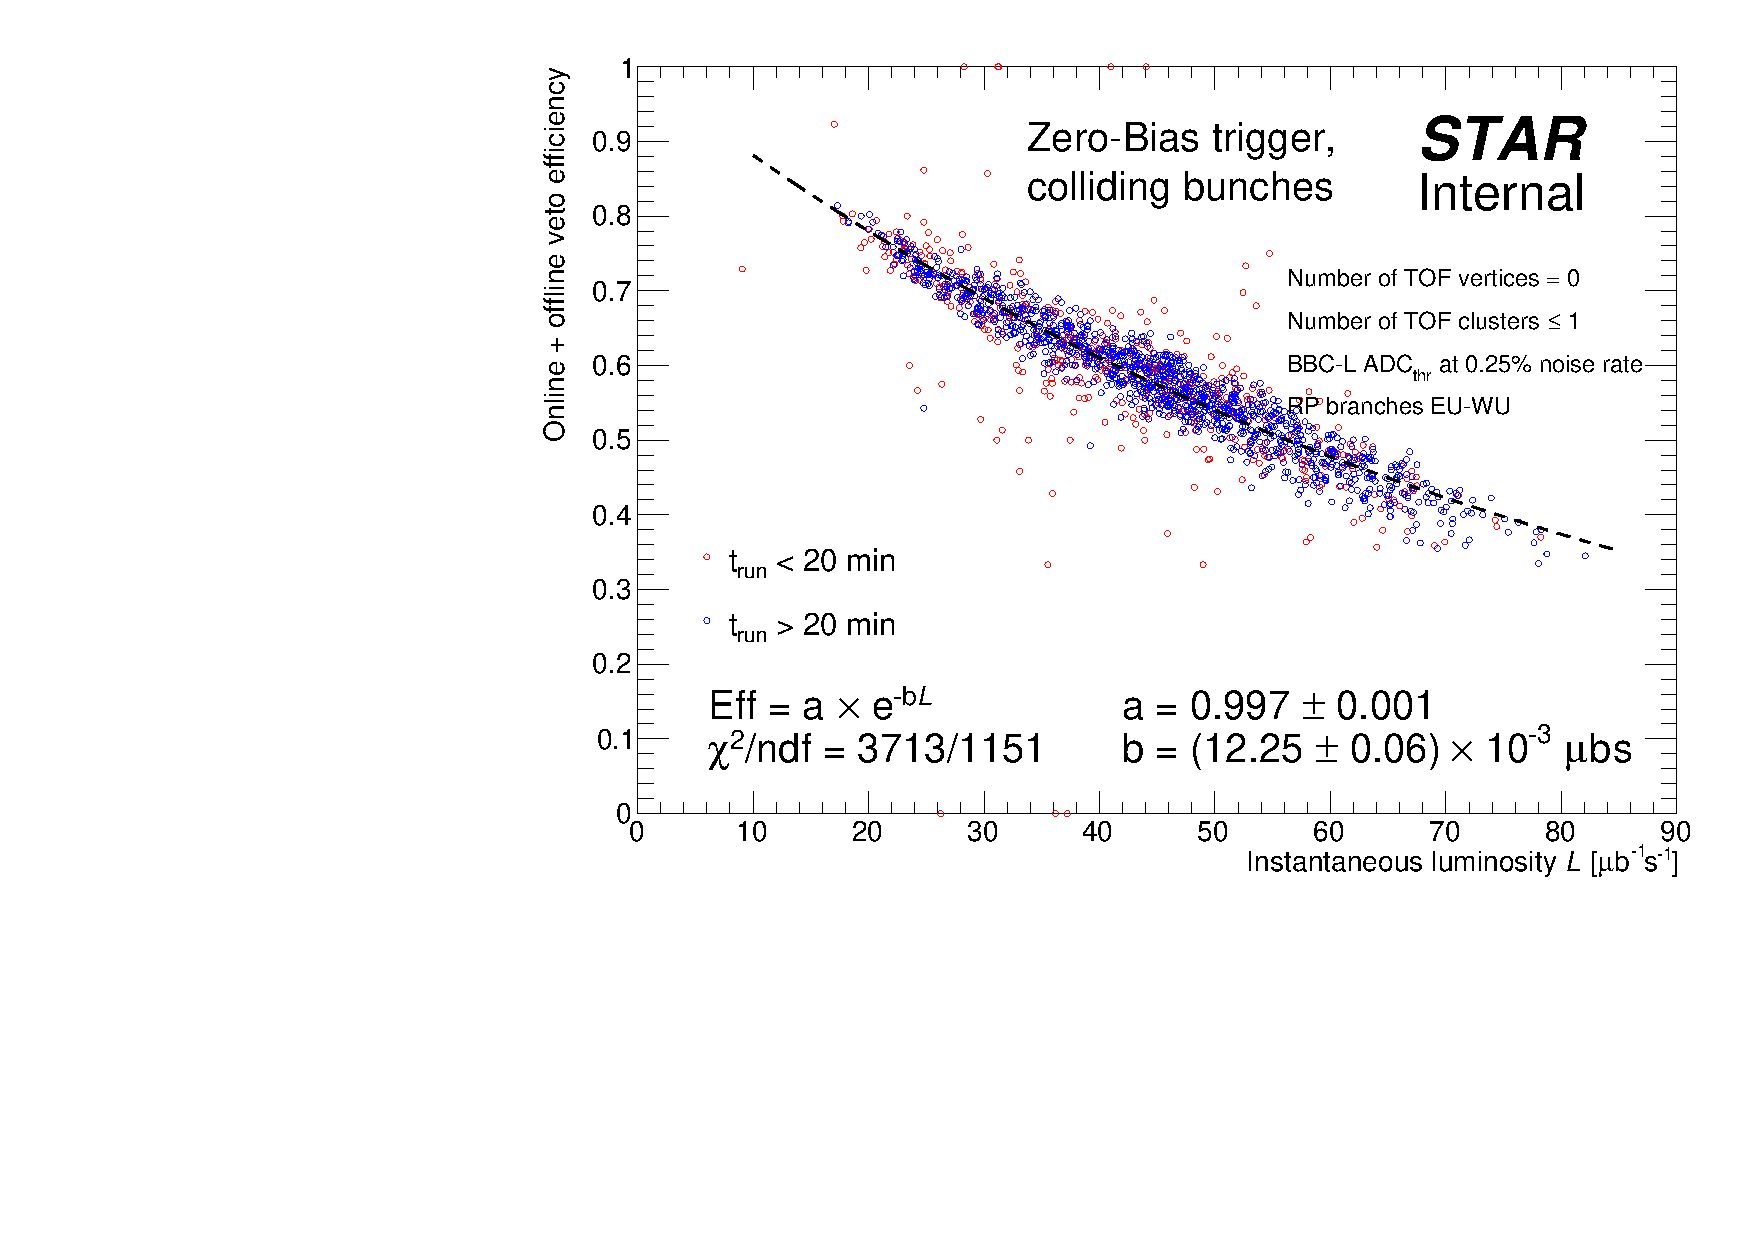
\includegraphics[width=\linewidth,page=1]{graphics/corrections/FullVetoEffVsInstLumi.pdf}}
  \end{subfigure}\\
  \begin{subfigure}[b]{\linewidth}\addtocounter{subfigure}{1}
                \subcaptionbox{\label{fig:sampleBbcSmallAdc}}{\includegraphics[width=\linewidth,page=3]{graphics/corrections/FullVetoEffVsInstLumi.pdf}}
  \end{subfigure}
}%
\quad\quad%
\parbox{0.4725\textwidth}{
  \centering
  \begin{subfigure}[b]{\linewidth}\addtocounter{subfigure}{-2}
                \subcaptionbox{\label{fig:sampleBbcLargeAdcVsTac}}{\includegraphics[width=\linewidth,page=2]{graphics/corrections/FullVetoEffVsInstLumi.pdf}}
  \end{subfigure}\\
  \begin{subfigure}[b]{\linewidth}\addtocounter{subfigure}{1}
                \subcaptionbox{\label{fig:sampleBbcLargeAdc}}{\includegraphics[width=\linewidth,page=4]{graphics/corrections/FullVetoEffVsInstLumi.pdf}}
  \end{subfigure}
}%
\caption[Overall efficiency of online and offlince cuts as a function of instantaneous luminosity.]{Overall efficiency of the online BBC-small, ZDC and ET\&IT trigger veto, primary vertices limit~(\ref{enum:CutPrimVx}), BBC-large veto~(\ref{enum:CutBbcLarge}) and TOF clusters limit~(\ref{enum:CutTofClusters}) as a function of instantaneous luminosity for all possible combinations of east and west RP branches. Red and blue points represent runs lasting for less and more than 20 minutes, respectively. Black dotted lines reprent fits of exponential functions to blue points.}\label{fig:onlineAndOfflineVetoEff}%
\end{figure}
%---------------------------



\subsubsection{Missing \texorpdfstring{$p_{T}$}{pT} cut~(\ref{enum:CutMissingPt})}
\subsubsection{Particle identification~(\ref{enum:CutPid})}\label{sec:pidEff}

Correction reflecting efficiency of identification requires good modeling of detector response in terms of $dE/dx$ and TOF time ($m^{2}$) measurement which were used for this purpose as described in Sec.~\ref{subsec:pidCuts}. In addition to this, significant number of simulated events is needed to reduce statistical uncertainties of efficiency. The former was provided by adjusting $dE/dx$ spectra from embedded MC to match the data, as elaborated in Chap.~7 of Ref.~\cite{supplementaryNote}. The latter, however, was not easy to achieve for exclusive $K^{+}K^{-}$ and $p\bar{p}$ whose identification is most challenging and information about identification efficiency is the most needed among studied species. Specially for study of particle (exlusive pair) identification a dedicated MC simulation was prepared.

This dedicated MC simulation was designed to work as follows (simulation of single exclusive event of predefined pair ID is described):
\begin{enumerate}
 \item The position of $z_{\text{vtx}}$ was drawn from predefined distribution.
 \item Kinematics of central state particles was set: momentum (magnitude) $p$, pseudorapidity $\eta$ and azimuthal angle $\phi$ of positive and negative charge particles were drawn from predefined distributions.
 \item Both particles were tested if doubled radius of curvature $R$ of associated track in the magnetic field ($B=0.5$~T) of the TPC ($R \propto p_{T}/B$) is smaller than the radius of TOF detector barell (assumed 212~cm). If not then event was skipped and procedure was restared (back to 1.).
 \item The particles were propagated from the vertex at $(0,0,z_{\text{vtx}})$ through the magnetic field of TPC using Newton's method with the time step (in the laboratory) equal 100~ps, corresponding to space step $<3$~cm.
 \item After step 4. the position of the TOF cell was known allowing to calculate the TOF path length $L$ between the vertex and position of the TOF hit. Also the TOF hit time $t$ was then known, further smeared by adding random number from normal distribution with mean at 0 and standard deviation $\sigma_{\text{TOF}}=100$~ps to account for the finite TOF time resolution. In addition to this, reconstructed tracks' momenta were defined as the true momenta smeared by 3\%, to account for finite TPC momentum resolution. At this stage it was possible to calculate $m^{2}_{\text{TOF}}$ using Eq.~\eqref{eq:mSquared}.
 \item The $dE/dx$ measurement was simulated.
\end{enumerate}

% For the purpose of presented analysis parameters of this distribution were set to match the data: $\langle z_{\text{vtx}}\rangle=0$ and $\sigma(z_{\text{vtx}})=50$~cm, as well as $z_{\text{vtx}}$ was required to lie within the analysis limits (cut~\ref{enum:CutZVx}).


% \begin{figure}[ht!]\label{fig:correlationsTofPathLength}
%   \centering
%   \begin{tabular}{@{}p{0.49\linewidth}@{\quad}p{0.49\linewidth}@{}}
%     \subfigimg[width=\linewidth,page=1]{~~~~~~~~~~~~~~~~~~~a)}{graphics/corrections/DEdxErrorVsTofPathLength.pdf}\label{fig:dEdxErrorVsTofPathLength} &
%     \subfigimg[width=\linewidth,page=1]{~~~~~~~~~~~~~~~~~~~b)}{graphics/corrections/Log2dxVsTofPathLength.pdf}\label{fig:Log2dEdxVsTofPathLength}
%   \end{tabular}
%   \caption[$dE/dx$ error vs. TOF path length and $\log_{2}(dx)$ vs. TOF path length for exclusive event candidates.]{Correlation between uncertainty of the natural logarithm of $dE/dx / (1~\text{keV/cm})$ and track TOF path length (\ref{fig:dEdxErrorVsTofPathLength}) and correlation between base 2 logarithm of $dx$ and track TOF path length (\ref{fig:Log2dEdxVsTofPathLength}). The distributions were obtained for the exclusive event candidates after full selection, with all three types of particle pairs combined.} 
% \end{figure}


%--------------------------- 
\begin{figure}%[ht!] 
\centering
\parbox{0.4725\textwidth}{
  \centering
  \begin{subfigure}[b]{\linewidth}{
                \subcaptionbox{\label{fig:dEdxErrorVsTofPathLength}}{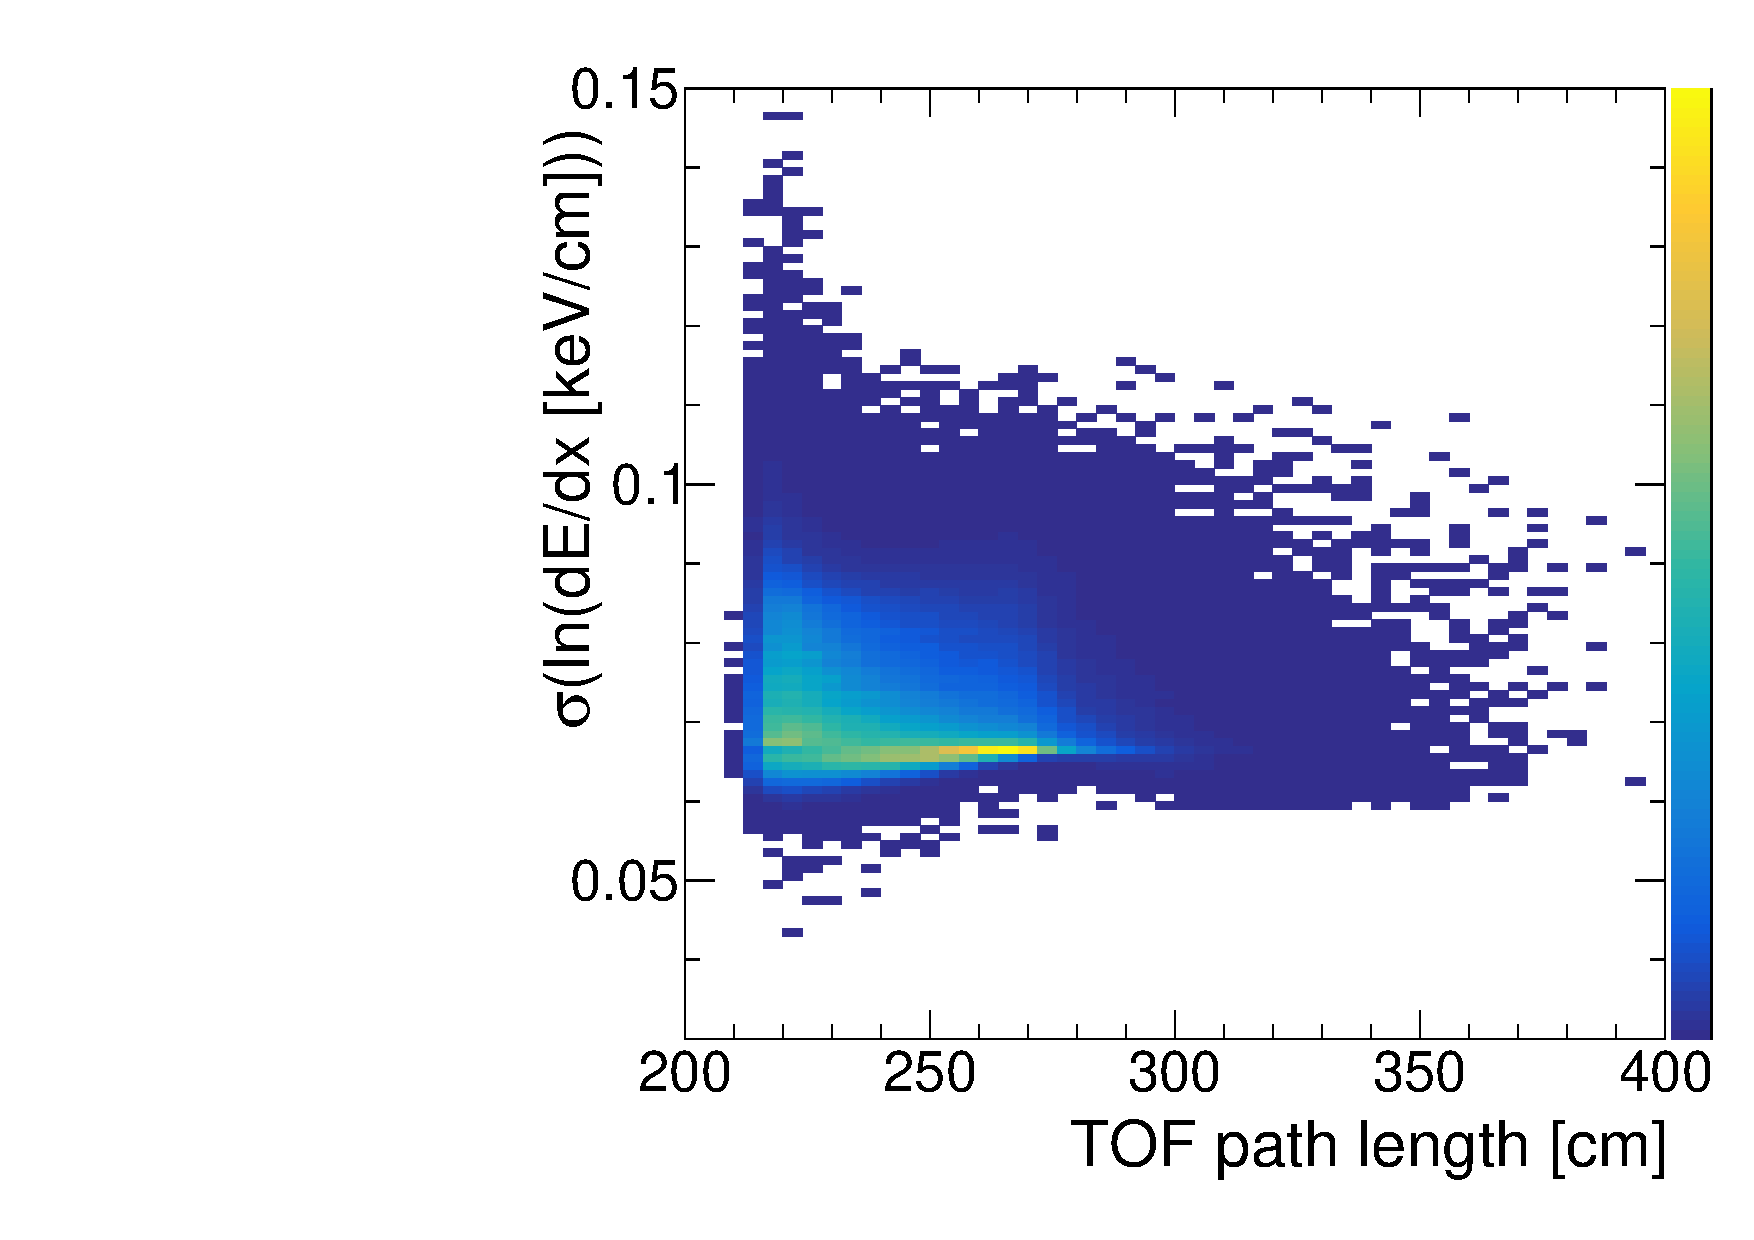
\includegraphics[width=\linewidth]{graphics/corrections/DEdxErrorVsTofPathLength.pdf}}}
  \end{subfigure}
}
\quad
\parbox{0.4725\textwidth}{
  \centering
  \begin{subfigure}[b]{\linewidth}{
                \subcaptionbox{\label{fig:Log2dEdxVsTofPathLength}}{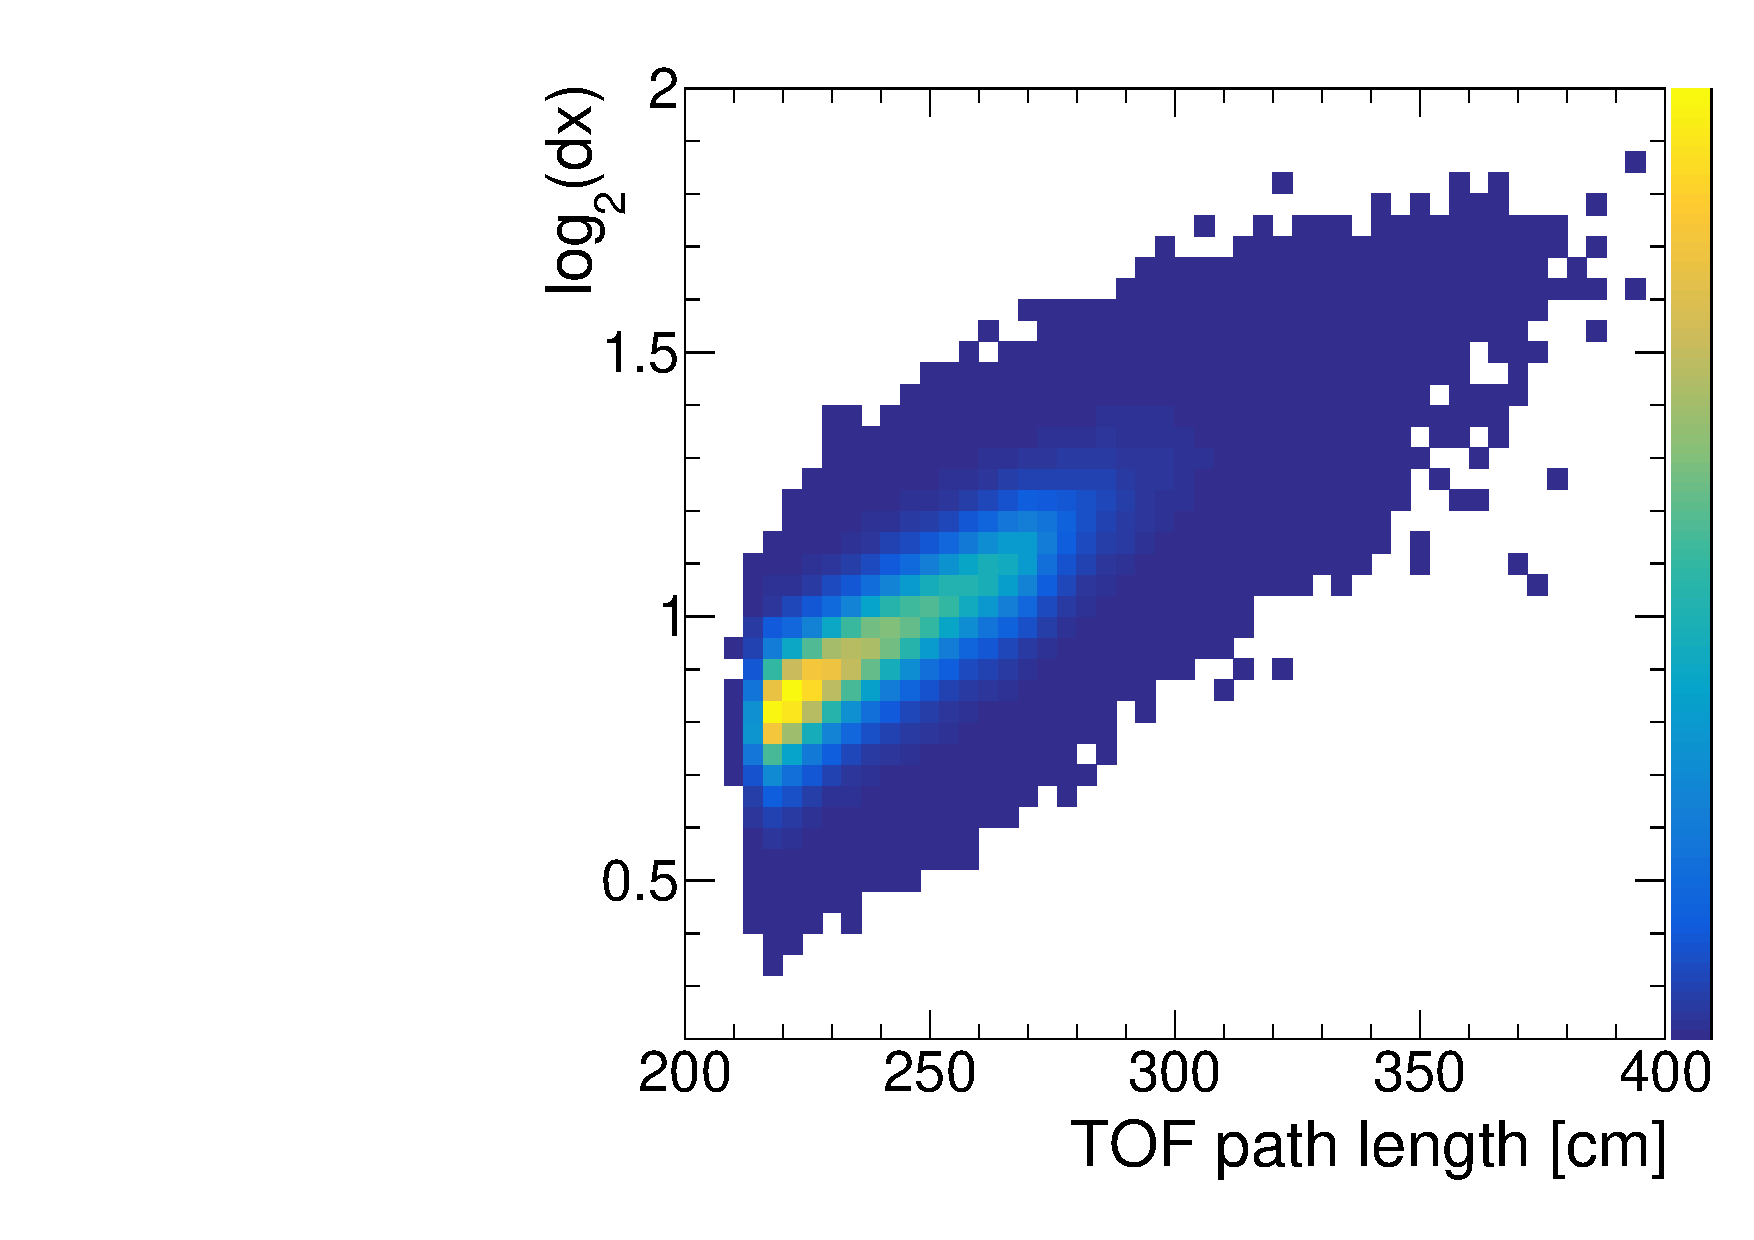
\includegraphics[width=\linewidth]{graphics/corrections/Log2dxVsTofPathLength.pdf}}}
  \end{subfigure}
}% 
\caption[$dE/dx$ error vs. TOF path length and $\log_{2}(dx)$ vs. TOF path length for exclusive event candidates.]{Correlation between uncertainty of the natural logarithm of $dE/dx / (1~\text{keV/cm})$ and track TOF path length (\ref{fig:dEdxErrorVsTofPathLength}) and correlation between base 2 logarithm of $dx$ and track TOF path length (\ref{fig:Log2dEdxVsTofPathLength}). The distributions were obtained for the exclusive event candidates after full selection, with all three types of particle pairs combined.} 
\end{figure}




\begin{figure}[ht!]\label{fig:pidEffVsPt}
  \centering
  \begin{tabular}{@{}p{0.315\linewidth}@{\quad}p{0.315\linewidth}@{\quad}p{0.315\linewidth}@{}}
    \subfigimg[width=\linewidth,page=1]{~~~~~~~~~~~~~~~~~~~~~~~a)}{graphics/corrections/EffVsPt.pdf} &
    \subfigimg[width=\linewidth,page=2]{~~~~~~~~~~~~~~~~~~~~~~~b)}{graphics/corrections/EffVsPt.pdf} &
    \subfigimg[width=\linewidth,page=3]{~~~~~~~~~~~~~~~~~~~~~~~c)}{graphics/corrections/EffVsPt.pdf} \\
    \subfigimg[width=\linewidth,page=4]{~~~~~~~~~~~~~~~~~~~~~~~d)}{graphics/corrections/EffVsPt.pdf} &
    \subfigimg[width=\linewidth,page=5]{~~~~~~~~~~~~~~~~~~~~~~~e)}{graphics/corrections/EffVsPt.pdf} &
    \subfigimg[width=\linewidth,page=6]{~~~~~~~~~~~~~~~~~~~~~~~f)}{graphics/corrections/EffVsPt.pdf} \\
    \subfigimg[width=\linewidth,page=7]{~~~~~~~~~~~~~~~~~~~~~~~g)}{graphics/corrections/EffVsPt.pdf} &
    \subfigimg[width=\linewidth,page=8]{~~~~~~~~~~~~~~~~~~~~~~~h)}{graphics/corrections/EffVsPt.pdf} &
    \subfigimg[width=\linewidth,page=9]{~~~~~~~~~~~~~~~~~~~~~~~i)}{graphics/corrections/EffVsPt.pdf}    
  \end{tabular}
  \caption[Pair identification efficiency and misidentification probability as a function of tracks' $p_{T}$.]{Pair identification efficiency (diagonal) and misidentification probability (off-diagonal) as a function of tracks' $p_{T}$ for $\pi^{+}\pi^{-}$, $K^{+}K^{-}$ and $p\bar{p}$ pairs. The results were obtained from the dedicated MC simulation described in the text. Blue lines and arrows mark the cut value on lower of the track $p_{T}$'s for kaons and protons.}
\end{figure}

%---------------------------









\subsection{RP track acceptance and reconstruction efficiency}\label{sec:rpAccAndEff}

To calculate RP acceptance and track reconstruction efficiency the embedded MC technique was used. The same sample was used as that described in Sec.~\ref{sec:rpDeadMat}, used for calculation of the dead-material related trigger veto.

The joint RP acceptance and track reconstruction efficiency for a given STAR side, $\mbox{\LARGE$\epsilon$}_{\text{RP}}^{\text{side}}$, was calculated as a probability that a single good quality RP track (satisfying cuts~\ref{enum:RpQualityCuts}-\ref{enum:RpLocalAngles}) matched with true-level primary forward proton is reconstructed on given side in the branch expected based on sign of $p_{y}$ of the proton, under condition that there is a trigger signal in that branch and there is no trigger signal in the other branch on the same side.

Technically the $\mbox{\LARGE$\epsilon$}_{\text{RP}}^{\text{side}}$ was obtained in the following procedure:
\begin{enumerate}
	\item It was verified if there is a trigger signal in the branch that the primary forward proton is expected to reach based on its $p_{y}$ ($p_{y}>0$ - branch UP, $p_{y}<0$ - branch DOWN). Additionally required lack of trigger signal in the other branch on the same side. These events formed $set~A$.
	\item The nominal RP track selection algorithm was used to find a single good quality track (cuts~\ref{enum:RpQualityCuts}-\ref{enum:RpLocalAngles}) on given side. If exactly one such track was found, it was additionally checked if it is matched with true-level primary proton. These events formed $set~B$.
	\item The efficiency was determined by the ratio of histograms from $set~B$ and $set~A$:
	\begin{equation}\label{eq:rpEffDef}
 \mbox{\LARGE$\epsilon$}_{\text{RP}}^{\text{side}}(p_{x}, p_{y}, z_{\text{vtx}}) = \mbox{\LARGE$\varepsilon$}\left(\RPSIDE\left|\TRSIDE\land~!\TRNSIDE\right.\right) = %
 \frac{(p_{x}, p_{y}, z_{\text{vtx}})~\text{histogram for protons from}~set~B}{(p_{x}, p_{y}, z_{\text{vtx}})~\text{histogram for protons from}~set~A}
  \end{equation}
	
\end{enumerate}

It should be noted that the momentum components $(p_{x}, p_{y})$ were taken from the proton with accounted effect of the beam divergence (after the original initial momentum smearing).

%---------------------------
\begin{figure}[ht!]%
\centering%
\begin{minipage}{.4725\textwidth}%
  \centering%
  \includegraphics[width=\linewidth,page=10]{graphics/corrections/mcFullEffPxPy.pdf}%
  \caption[Sample RP track reconstruction efficiency in a single $z$-vertex bin.]{Sample RP track reconstruction efficiency in a single $z$-vertex bin on the east STAR side. The efficiency was calculated using forward proton MC simulation embedded into zero-bias data. Green envelopes mark the fiducial region of the measurement, while dashed yellow lines mark the part of the fiducial region with a data-driven efficiency correction needed, as explained in Sec.~10.3.1 of Ref.~\cite{supplementaryNote}.}\label{fig:rpEffSample}
\end{minipage}%
\quad\quad%
\begin{minipage}{.4725\textwidth}%
  \centering
  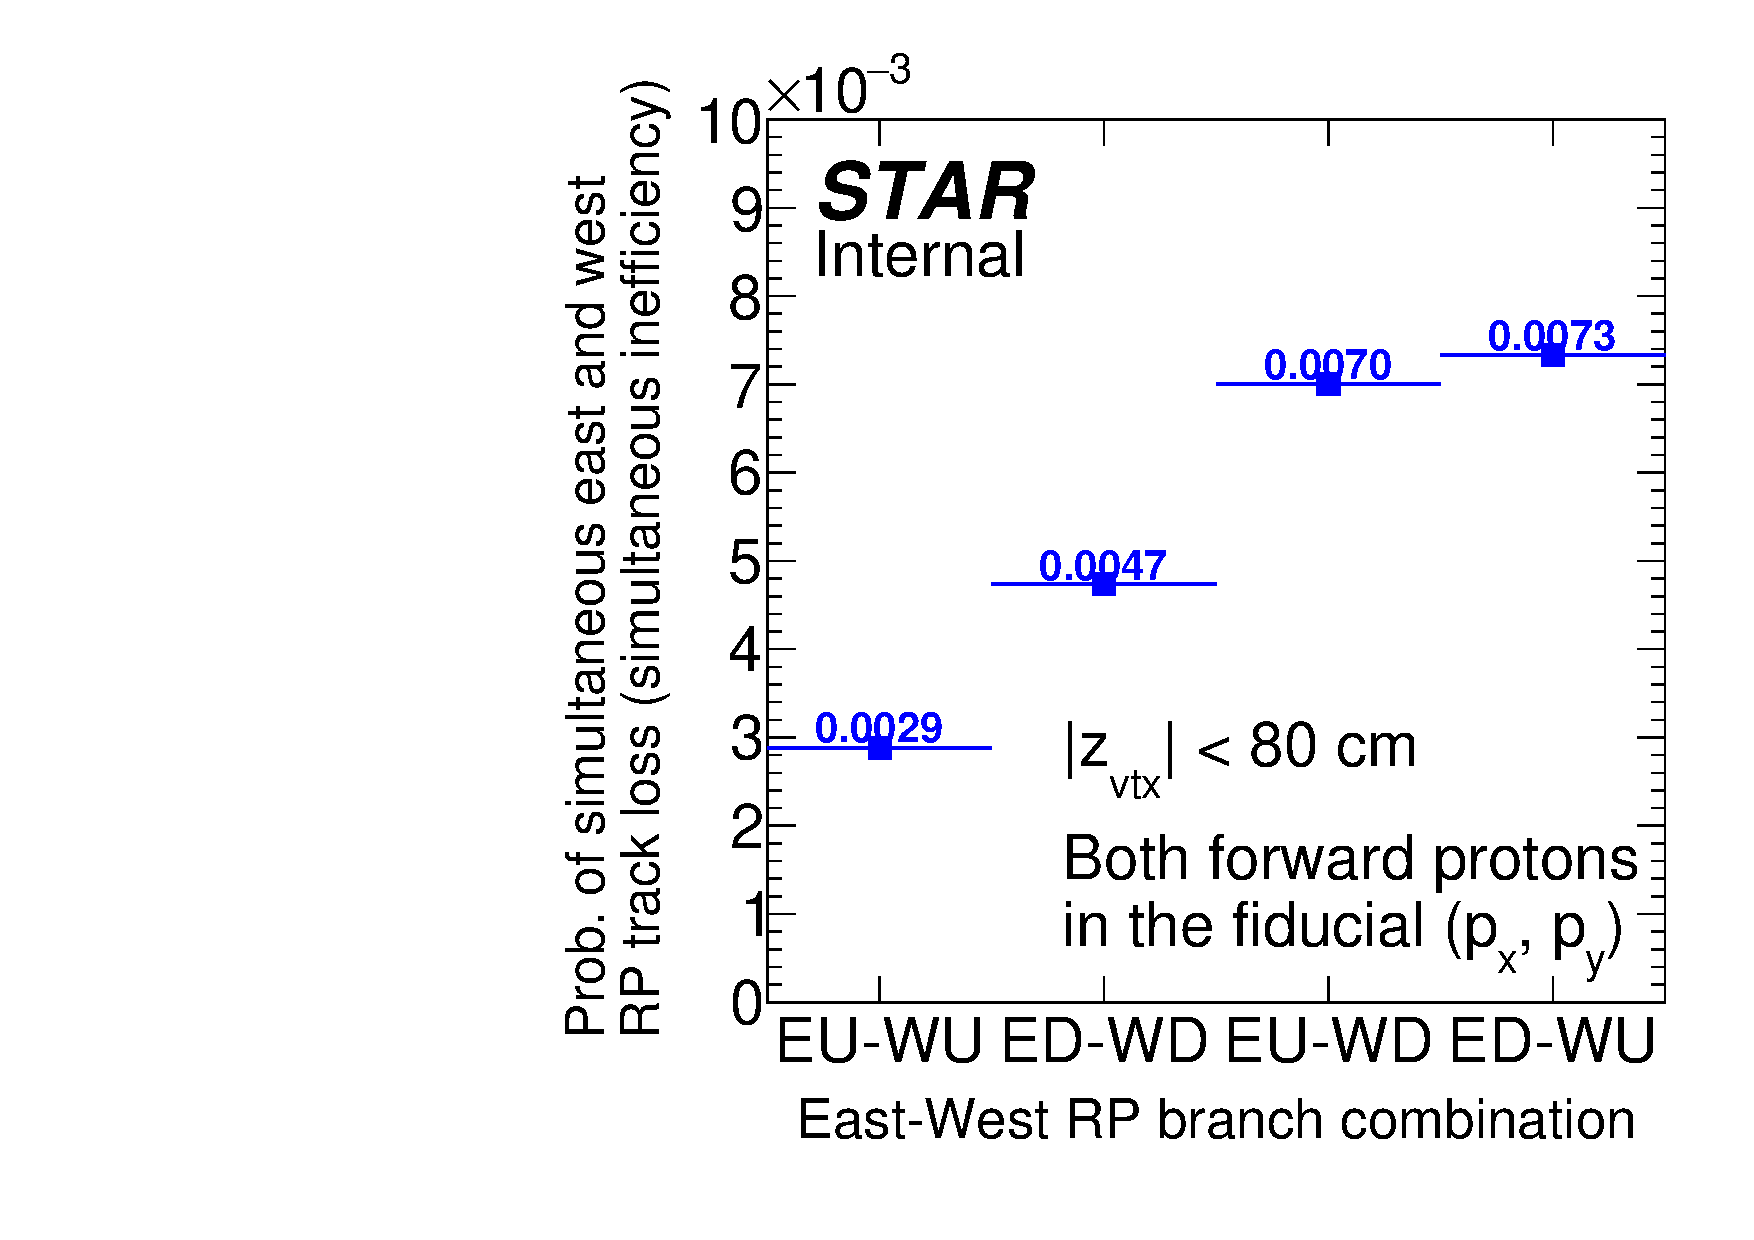
\includegraphics[width=\linewidth]{graphics/corrections/SimultaneousEastWestRpTrackLoss.pdf}%
  \caption{Probability of simultaneous inefficiency of the RP track reconstruction calculated from the CEP MC embedded into zero-bias data.\newline\newline\newline\newline\newline}\label{fig:SimultaneousEastWestRpTrackLoss}
\end{minipage}%
\end{figure}%
%---------------------------


The efficiency calculated in the way described above is, by design, the acceptance, reconstruction and selection efficiency for a single proton on one side of the IP. In CEP event there are two independent forward protons which may be simultaneously not reconstructed or rejected by the selection algorithm due to e.g. elastic pile-up interaction providing additional good quality proton tracks on both sides of IP. One could, in principle, calculate 5-dimensional efficiency for both forward protons (in variables $p_{x}^{\text{E}}, p_{y}^{\text{E}}, p_{x}^{\text{W}}, p_{y}^{\text{W}}$ and $z_{\text{vtx}}$) which would ultimately account for the simultaneous east and west inefficiency, however this would require orders of magnitude larger statistics of MC to provide reasonably low statistical uncertainty of the efficiency. Instead, on top of the 3-dimensional reconstruction and selection efficiencies for east and west RPs we calculate (from embedded MC) probability that the proton tracks are simultaneously not reconstructed or selected on the east and west side, despite the trigger signal solely in expected RP branches (no trigger veto) and true-level $(p_{x}, p_{y})$ of both forward protons contained in the fiducial region. This probability, denoted as
\begin{equation}
\mathcal{P}^{\text{E\&W}}_{\text{loss}} = \mbox{\LARGE$\varepsilon$}\left(!\RPE\land~!\RPW\Big|\TRE\land\TRW\land~!\V\Big.\right),
\end{equation}
 is presented in Fig.~\ref{fig:SimultaneousEastWestRpTrackLoss} for all four comibnations of east and west RP branches.





\subsection{TPC vertex reconstruction efficiency}\label{sec:tpcVxRecoEff}

%---------------------------
\begin{wrapfigure}{o}{0.365\textwidth}\vspace*{-9pt}
  \centering
  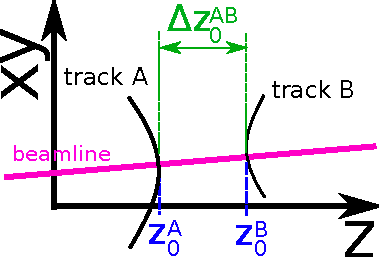
\includegraphics[width=0.365\textwidth]{graphics/corrections/deltaZ0Definition2.pdf}
  \caption[Sketch with definition of $\Delta z_{0}$.]
   {Sketch with definition of the longitudinal separation of two tracks (helices) $\Delta z_{0}$.}
   \label{fig:deltaZ0Sketch}\vspace*{-9pt} 
\end{wrapfigure}
%---------------------------

The definition of vertex reconstruction efficiency ($\mbox{\LARGE$\epsilon$}_{\text{vtx}}$) established in this analysis is the probability that two global tracks, both associated with true-level primary particles from the kinematic region of the measurement, both satisfying kinematic and quality criteria (cuts~\ref{enum:TpcKinematicCuts} and ~\ref{enum:TpcQualityCuts}) and both matched with hits in TOF, form a vertex listed in the collection of reconstructed primary vertices and DCA(R) and DCA(z) of both global tracks calculated w.r.t. this vertex is contained within the limits of cut~\ref{enum:TpcDcaCuts}.

We calculated this efficiency as a function of the longitudinal separation between two tracks (global helices) $\Delta z_{0}$. Illustration of this quantity is given in Fig.~\ref{fig:deltaZ0Sketch}. We consider this a natural quantity to present the vertexing efficiency - the closer to each other the helices are on the beamline, the more probable it is that two tracks will form a common primary vertex. It is in accordance with the way the vertexing algorithm works.


The vertexing efficiency was calculated from the data in the following way:
\begin{enumerate}
\item Data from RP\_CPT2 trigger were used. Events were selected with nearly the same cuts as in nominal CEP analysis (Sec.~\ref{sec:listOfCuts}). The requirement of exactly one primary vertex with exactly two primary TOF tracks was dropped. Instead, analysis utilized only global TOF tracks - exactly two global TOF tracks were required (cut~\ref{enum:TpcTofMatched} without primary track requirement), passing also cuts~\ref{enum:TpcOppoSign}-\ref{enum:TpcQualityCuts}. In this case the position of the vertex was reconstructed as\vspace*{-10pt}
\begin{equation}
 z_{\text{vtx}} = \frac{z_{0}^{+}+z_{0}^{-}}{2},\vspace*{-5pt}
\end{equation}
where $z_{0}^{+}$ and $z_{0}^{-}$ are longitudinal impact parameters ($z$-coordinates of points of closest approach to the beamline) of positive and negative charge particle tracks, respectively. The vertex position was normally required to satisfy cut~\ref{enum:CutZVx}. Events after full selection, classified as exclusive $\pi^{+}\pi^{-}$ candidates, formed $set~A$.

\item The two global TOF tracks were checked if they have associated primary tracks, and the two primary tracks are assigned to the same primary vertex. If yes, the tracks were additionally subjected to cut~\ref{enum:TpcDcaCuts}. Events passing descibed selection formed $set~B$.

	\item The efficiency was determined by the ratio of histograms from $set~B$ and $set~A$:
	\begin{equation}\label{eq:vertexingEffDef}
 \mbox{\LARGE$\epsilon$}_{\text{vtx}}(|\Delta z_{0}|) = \frac{|\Delta z_{0}|~\text{histogram for events from}~set~B}{|\Delta z_{0}|~\text{histogram for events from}~set~A}.
  \end{equation}
\end{enumerate}

Distribution of $|\Delta z_{0}|$ between two CEP global track candidates after full selection ($set A$) is presented in Fig.~\ref{fig:deltaZ0}. The vertexing efficiency obtained with described method is shown in Fig.~\ref{fig:vertexingEff}. Solid green points represent efficiency calculated with the non-exclusive background preserved, while open black points represent efficiency with this background subtracted (using method described in Sec.~\ref{sec:bkgdSubtraction}). Since the vertexing efficiency does not depend on the physics process and background is purely of physics origin the black and green points should overlap. Such picture emerges from presented comparison. We have calculated the same efficiency using CEP MC embedded into zero-bias data, the result is shown in Fig.~\ref{fig:vertexingEff} with red points. There is very good agreement between vertexing efficiency in the data and embedded MC for $|\Delta z_{0}|<1$~cm, where most ($\sim80\%$) of the signal is present. The differences in high-$|\Delta z_{0}|$ tail are understood as a result of the imperfect description of the pointing resolution (here: the transverse resolution) of TPC tracks in STARsim. Although the pointing resolution is adjusted to gain more accurate description of the data by MC simulation as described in Chapter~8 of Ref.~\cite{supplementaryNote}, this does not help with the vertexing which is performed at the level of raw data (MC) processing to MuDst. Another reason could be different $p_{T}$ (thus also $d_{0}$) spectrum of CEP tracks in the data and MC (GenEx).

%---------------------------
\begin{figure}[ht!]%
\centering%
\begin{minipage}{.4725\textwidth}%
  \centering%
  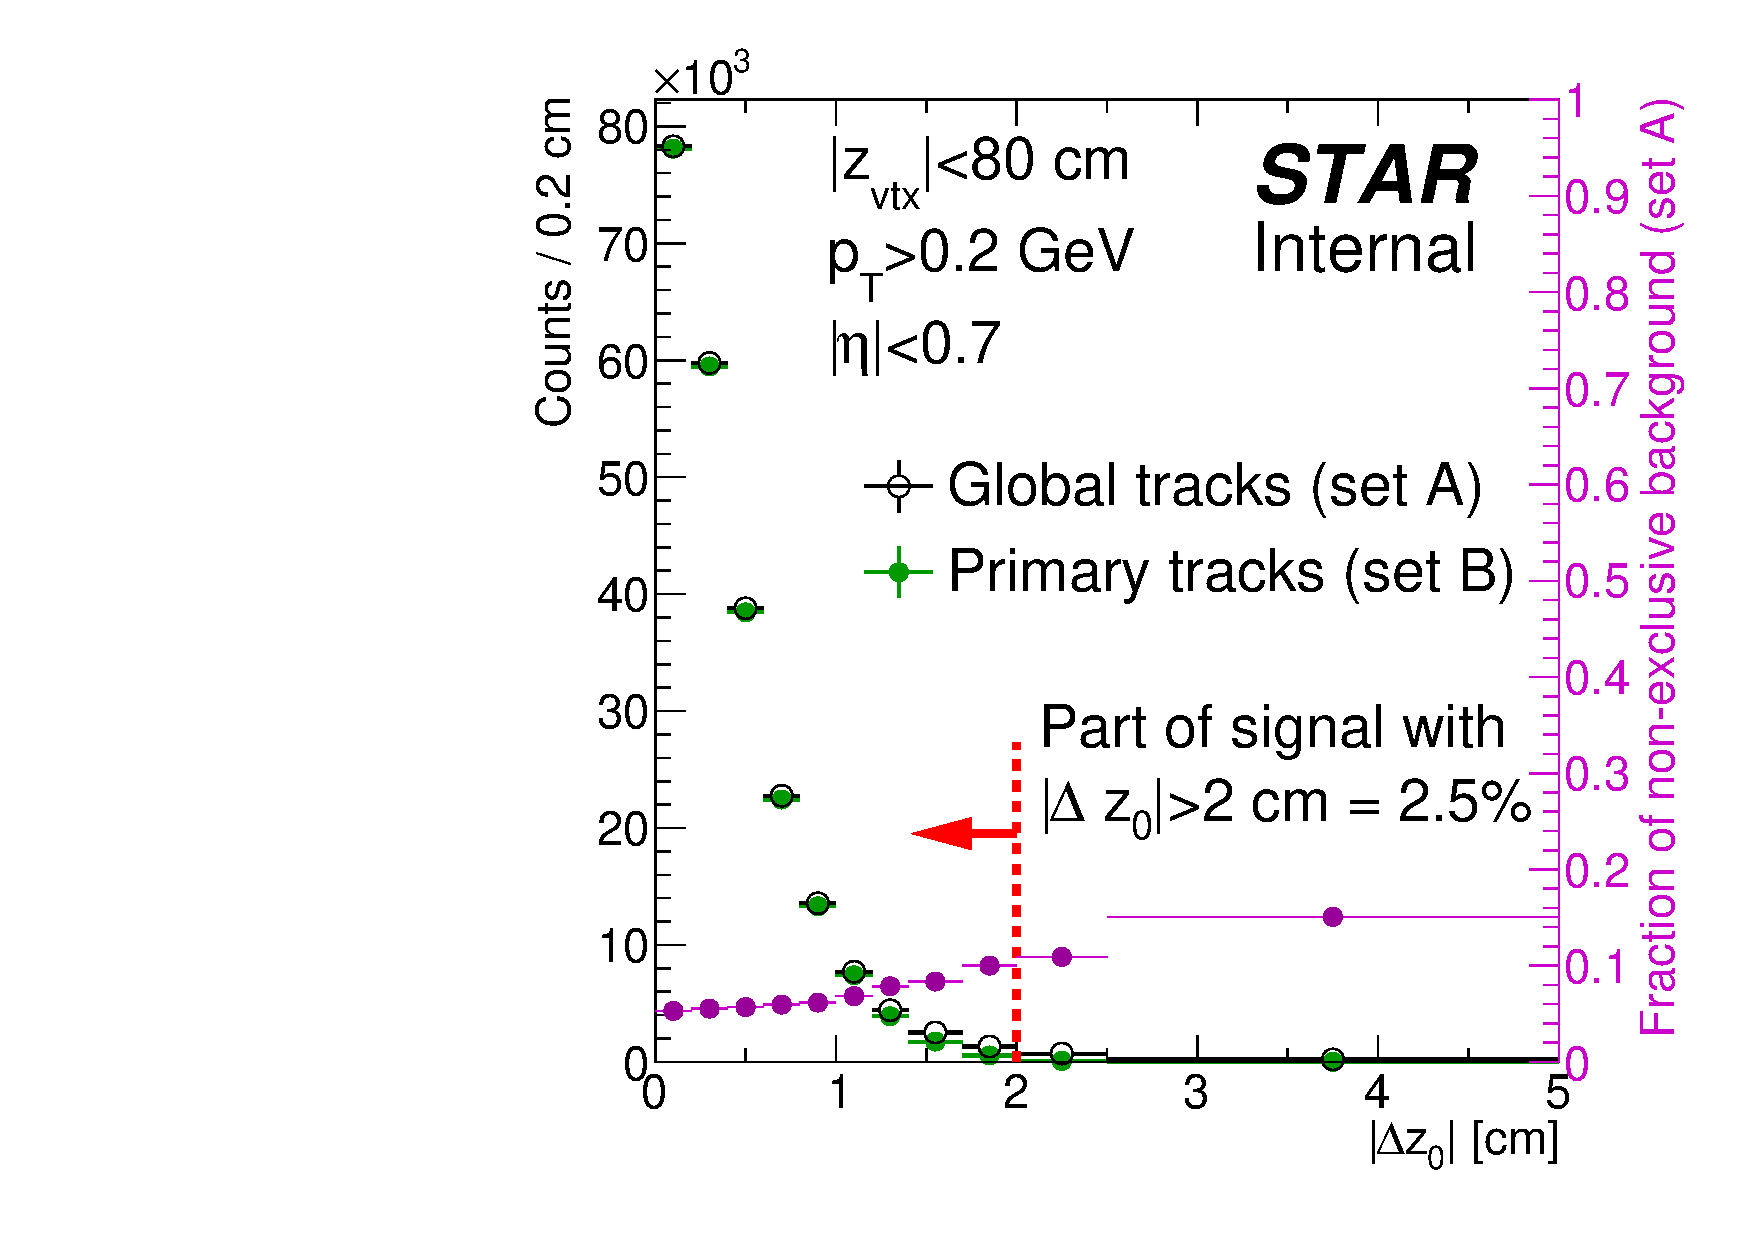
\includegraphics[width=\linewidth]{graphics/corrections/DeltaZ0WithBackground.pdf}%
  \caption[Distribution of $\Delta z_{0}$ together with fraction of non-exclusive background.]{Distribution of $\Delta z_{0}$ between two CEP-candidate global tracks (green and black points) together with fraction of non-exclusive background in black distribution as a function of $\Delta z_{0}$ (violet points).}\label{fig:deltaZ0}
\end{minipage}% 
\quad\quad%
\begin{minipage}{.4725\textwidth}%
  \centering
  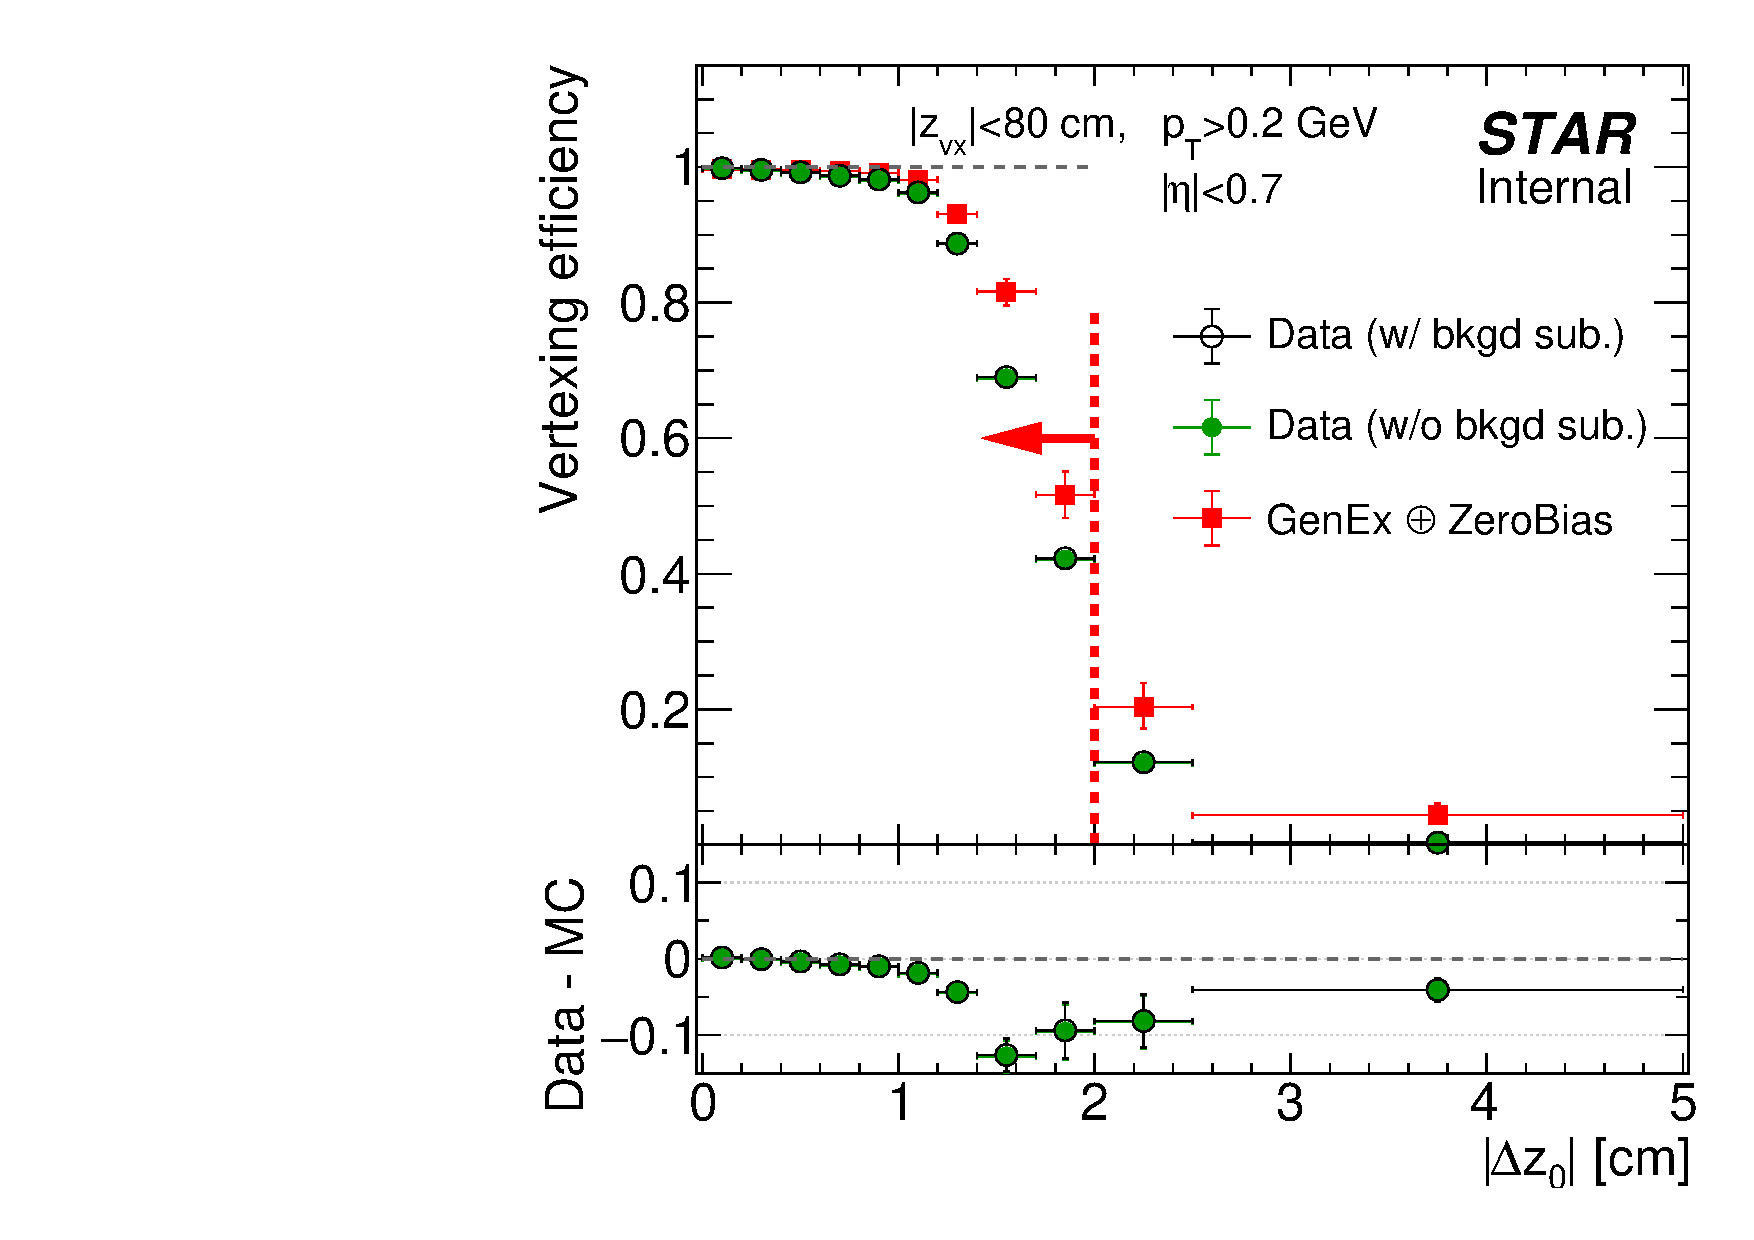
\includegraphics[width=\linewidth]{graphics/corrections/VertexingEfficiency.pdf}%
  \caption[Vertexing efficiency.]{Vertexing efficiency calculated from the data (open black and full green points) and from embedded MC (red points) as a function of $\Delta z_{0}$ between two CEP-candidate global tracks.}\label{fig:vertexingEff}
\end{minipage}%
\end{figure}%
%---------------------------

Based on the width of $|\Delta z_{0}|$ distribution, the background content as a function of $|\Delta z_{0}|$, and the value of $\mbox{\LARGE$\epsilon$}_{\text{vtx}}$ as a function of $|\Delta z_{0}|$, we decided to accept in analysis only tracks which satisfy $|\Delta z_{0}|<2$~cm. This assures that the vertexing efficiency does not drop below $\approx 30\%$, as well as it coincides with the primary tracks requirement of $|\text{DCA}(z)|<1$~cm. In the correction procedure we nominally use the vertexing efficiency represented by open black points in Fig.~\ref{fig:vertexingEff} (to correct the MC e.g. in closure tests we use red points instead). The additional correction factor connected with the cut on maximum $|\Delta z_{0}|$ (2~cm) was calculated from the data and equals $2.4\%$ (Fig.~\ref{fig:deltaZ0}). This correction is used as an additional normalization correction factor, which is different from $\mbox{\LARGE$\epsilon$}_{\text{vtx}}(|\Delta z_{0}|)$ applied in form of a weight to each selected CEP event.


\section{Particle energy loss}\label{sec:energyLoss}

Energy loss correction as a function of reconstructed particle $p_{T}$ in bins of $z$-position of reconstructed vertex has been calculated and presented in Chapter~5 of Ref.~\cite{supplementaryNote} for all analyzed particle species and both positive and negative charges. The correction was applied independetly for each particle in the following procedure:

\begin{enumerate}
	\item After central particles were identified (cut~\ref{enum:CutPid}) an absolute value of the particle transverse momentum correction ($-\Delta p_{T} = p_{T}^{\text{meas}}-p_{T}^{\text{true}}$) was read from the histogram corresponding to reconstructed $z_{\text{vtx}}$ and to assigned particle ID (Appendix~C of Ref.~\cite{supplementaryNote}).
	\item The momentum correction factor $f_{p}^{\text{corr}}$ was calculated:
	\begin{equation}\label{eq:pCorrFactor}
 f_{p}^{\text{corr}} = \frac{p_{T}^{\text{meas}} + \Delta p_{T}}{p_{T}^{\text{meas}}}.
  \end{equation}
  \item New, corrected momentum $\vec{p}^{corr}$ was assigned to the particle:
  \begin{equation}
   \vec{p}^{~\text{corr}} = f_{p}^{\text{corr}} \cdot \vec{p}^{~\text{meas}}.
  \end{equation}
  In this way all three components of particle momentum are corrected so that the pseudorapidity of a particle remains unchanged.
\end{enumerate}
This new momentum was further used in determination of total transverse momentum of all reconstructed particles, $p_{T}^{\text{miss}}$, as well as in applying TPC and TOF efficiency corrections and preparing histograms (cross sections) of physics quantities (e.g. invariant mass, rapidity of a pair of central tracks).


\section{Background subtraction}\label{sec:bkgdSubtraction}
% \section{Unfolding}\label{sec:unfolding}

% 
%   W analizie CEP wydajnosc werteksowania to prawdopodobieństwo że
%  oba pierwotne slady z punktu B tworza werteks (to znaczy sa na liscie
%  sladow primary wspolnego werteksu i spelniaja ciecia DCA).
%  Nie patrzymy na dodatkowe werteksy, hity w TOF, BBC_small
% 
% E) --- pozostale wydajnosci
% 
%   w przypadku analizy CEP jest to pile-up czyli dodatkowy werteks lub
%   dodatkowy hit w TOF lub sygnal w BBC. Te poprawk mamy z embeddingu
%   patrzac ile przypadkow z D ma dodatkowy werteks, hist w TOF lub BBC
% 
%   To samo powinnismy dostac z analizy "naszych" zero-bias.
% 
%   W przypadku analizy SD mamy pile-up czyli dodatkowy werteks, BBC
%   po stronie protonu też to znamy z embeddingu lub "naszych" zero-bias.
% 
%   Dodatkowo dochodza dodatkowe werteksy z oddzialywań wtornych/rozpadow.
%   Ten efekt znamy z MC. Powinno byc to samo z pile-up'em jak i  bez
% 
% 
% Jakies uwagi?
